\documentclass[11pt]{article} 

\usepackage{fullpage}
\usepackage[top=1.5cm, bottom=1.5cm, left=2cm, right=2cm]{geometry}
 \usepackage{array,multirow,graphicx}
 \usepackage{float}
 \usepackage{comment}
  \usepackage{xcolor}


\begin{document}
\title{Preliminary research Playaprinter 3D Nozzle}
\author{Thomas Martens Tia2}
\date{\today}
\maketitle

\begin{figure}[hbtp]
\caption{playaprinter}
\centering
\includegraphics[scale=0.50]{Playaprinter.png}
\end{figure}
\newpage

\tableofcontents

TO DO: bronnen plaatsen\\
		Onderzoek naar Endstops als extra hoofdstuk????
		onderzoek naar 8 bit vs 32 bit controllers
		
		
		
\newpage


\section{Introduction Playa Project//ISSUE/Probleemstelling}
In our daily lives we use normal printers that can print the design on a flat surface, a 3D printer and  a ordinary  printer  working  principle  is  basically the  same, just  some  different  printing materials. Printing material  for a ordinary  printer  is ink  and  paper. A 3D  printer can be equipped  with metal, ceramic, plastic, sand and  other  different  print  materials.  The  printer  is  connected  to  the  computer through  USB/Bluetooth through which it prints layers of material. The methods generally referred to as 3D printing is called fused deposition modeling(FDM).\\

In this research paper  we shall examine the feasibility of creating a 4 by 4 meter 3D printer. This project is a collaboration between the Hogeschool Rotterdam and Havenlab RDM. It started at a Burning Man Festival with the idea to create a 3D printer that would "leave no Trace". The components of the Playaprinter needed to be crafted of parts that are available to the general public. Furthermore the design/code needs to be based off FOSS(free and open-source software). The "Leave no Trace" refers to the fact that the 3D printer could use natural resources like clay to create structures/sculptures. \\

Against this background, the central question that motivates this paper will be if it is possible to create a open source 'DIY' print nozzle. It is the most crucial part for creating precise 3D structures. In this paper we look at the different kind of 3D printer nozzles and how the work. In addition if it is possible to create a 3D printer nozzle and other needed materials that are available to the general public.  \\


\newpage


\section{Different materials used in 3D printing}	
One of the most crucial factors in creating your own 3D printer is knowing the type of material being used. This determines the 3D head that is needed to transport/heat the substance. To answer this question, we begin by taking a closer look at the different kind of materials. 

\subsection{ABS - PLA - PTG}
			
	The most common type of 3D print material found in almost every consumer device. It is easily  accessible and works well in different situations depending on the type 3D filament. Some filament can make a 3D structures flexible while others filaments excel at strength and pressure. ABS was one of the first plastic to be used with 3D printers. Many years later, ABS is still a very popular material thanks to its low cost and good mechanical properties. ABS is known for its toughness and impact resistance, allowing you to print durable parts that will hold up to extra usage and wear.  \\
	
\begin{figure}[hbtp]
\caption{Common 3D printer material}
\centering
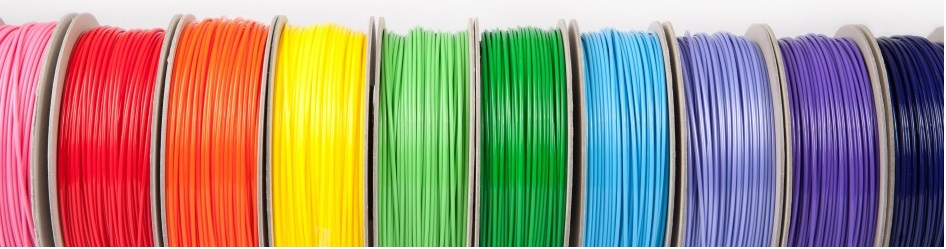
\includegraphics[scale=0.5]{3dmaterials.png}
\end{figure}

	
\subsection{Algae}    
	Algae is a new 3D print material first proofed by researchers at the Wageningen University. Working with scientists, Klarenbeek  developed a new way of 3D printing with living organisms. The created a 3D printed chair using living fungus, which then grows inside the structure to give it strength.  A different version of this is growing algea and than process the algae into a special sustainable filament.\\
	
	\begin{figure}[hbtp]
	\caption{Algea \& 3D Filament}
	\centering
	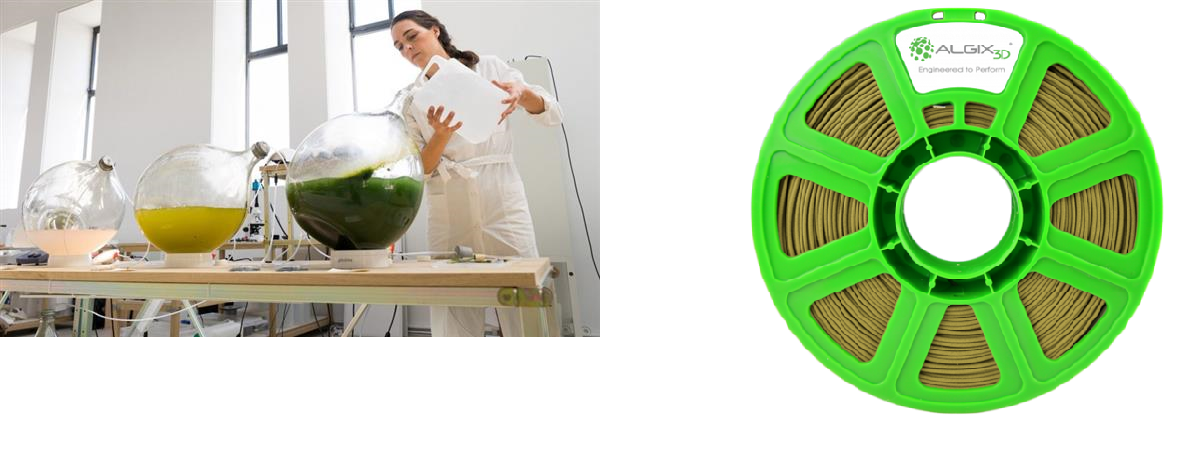
\includegraphics[scale=0.5]{algea.png}
	\end{figure}
	
\newpage

\subsection{Clay and other  sand combinations}

	 Clay is a common resource that can be found almost anywhere, it is a finely-grained natural rock or soil material that combines one or more clay minerals. Clay are plastic due to particle size and geometry as well as water content. A property of clay is that it become hard, brittle and non–plastic upon drying or heating. In the natural environment a lot of different combinations of sand, silt and other materials can be found. Clay is distinguished from other fine-grained soils by differences in size and mineralogy.\\
	
	\begin{figure}[hbtp]
	\caption{Building Clay \& Natural Clay }
	\centering
	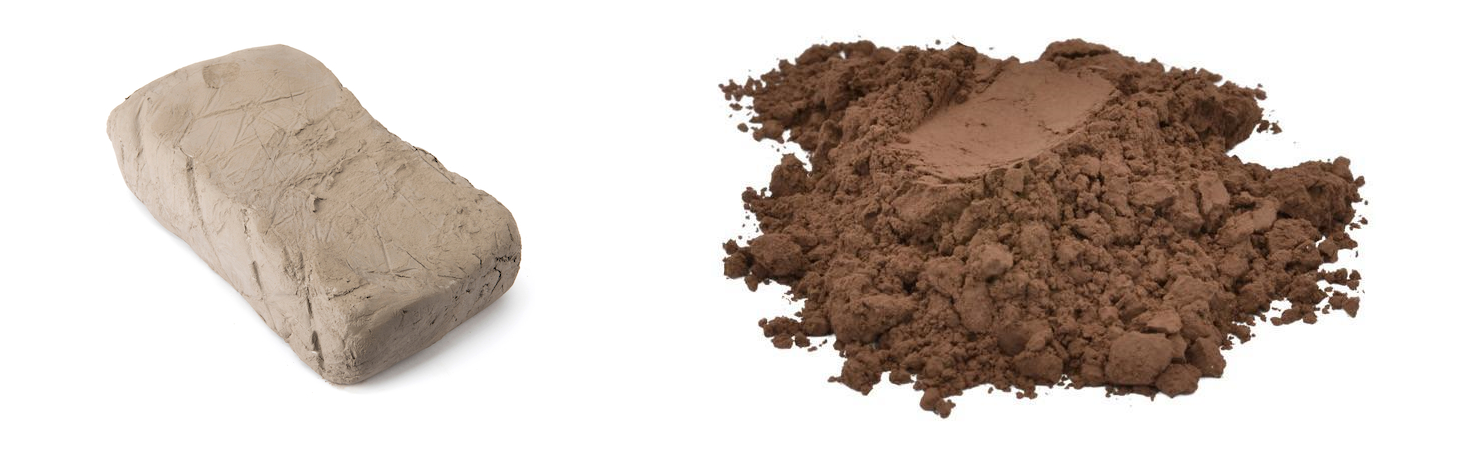
\includegraphics[scale=0.45]{clayTotal.png}
	\end{figure}

	
	\subsection{Metal powders}
		Metal 3D printing is carried out by fusing powdered metal particles together to create a object in a successive layer by layer printing process. Metal is heated up and requires specialized equipment to create special 3d metal powder. A powder bed fusion 3D printer uses a laser to sinter powdered material. A powerful laser beam selectively melts and fuses tiny powder particles together. Once a layer is finished, more powder is rolled and spread onto the print bed. The particle properties of the metals is very important for successful 3D printing.\\
		
		
\begin{figure}[hbtp]
\caption{Metal Powder}
\centering
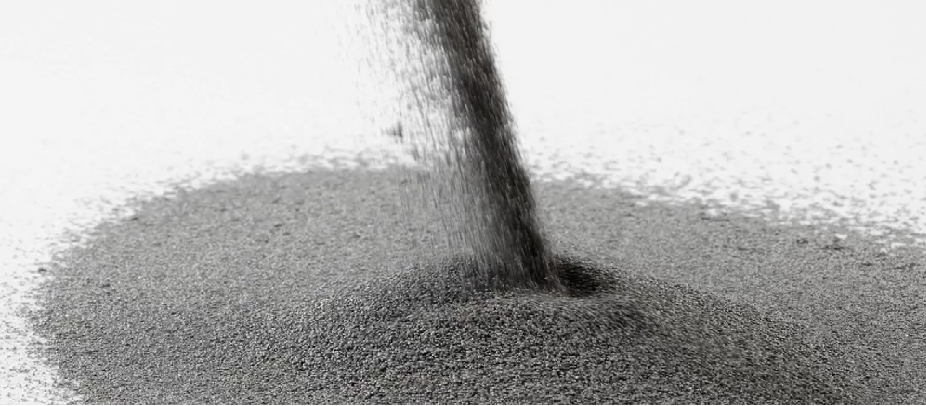
\includegraphics[scale=0.30]{powder.png}
\end{figure}

\newpage


All these different types of materials require a specific type of 3D nozzle + extruder combination to work. ABS \& Alga and other common filament uses a more traditional hotend to create 3D objects.  For clay and other natural resources this usually  requires a auger design with a fluid pump to work correctly. This is due to the fact that it needs a container and controlled pressure.\\

Industrial installation uses metal powder to use as a base material for printing. In the next chapter the paper will look at the different kind of systems in greater detail.  

\newpage
\section{Printhead}

In this section we will look at the different 3D nozzle \& extruders combinations and the working principles behind them. Our focus is on the possibly to replicate it with normal means and being applicable for the (PlayaPrinter) 4m by 4m printer. 



\subsection{Hotend Design}

The hotend the is most common used in a 3D printer. The hotend is where the heated filament comes 
out and moves through the nozzle to the print bed to create a 3D object. The heaterblock is the part that is responsible for heating up the filament. ABS needs to be around 230 degrees to start to liquefy. During the liquefaction stage the filament is compressed in smaller space to increase heat friction. Temperature control is a big factor for creating good 3D print results. 

\begin{figure}[hbtp]
\caption{Hotend }
\centering
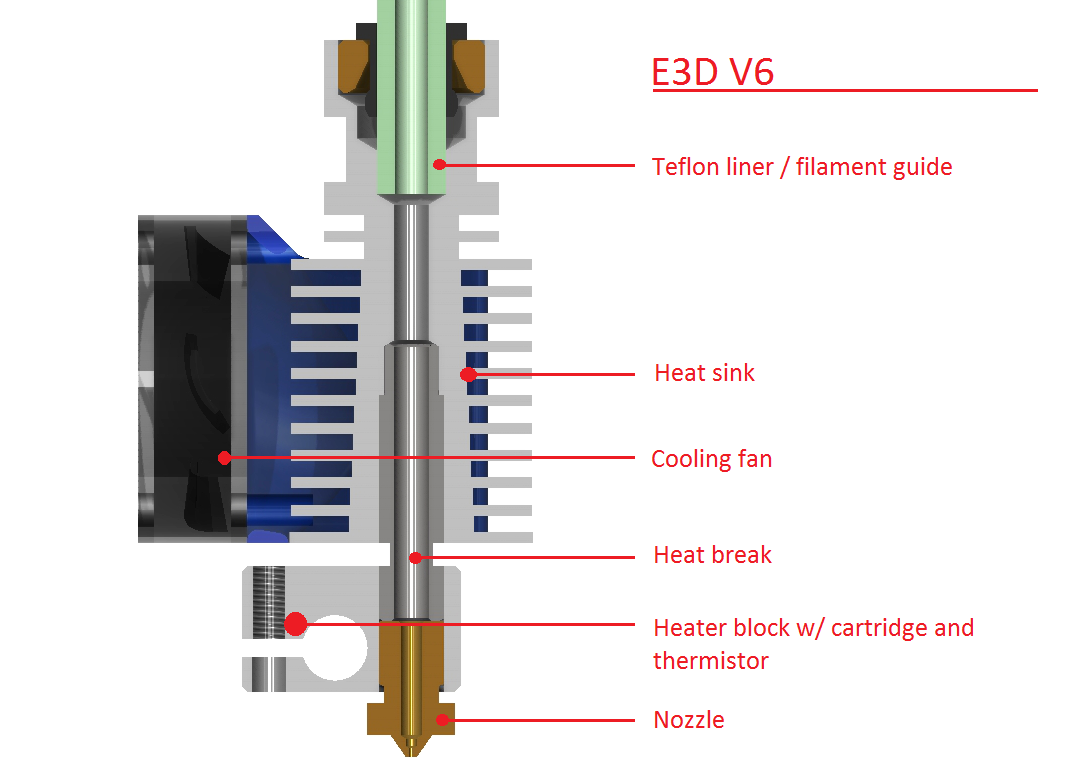
\includegraphics[scale=0.30]{hotend.png}
\end{figure}

\subsection{Stereolithography  } 
The stereolithography  process first appeared in the early 1980s, when Japanese researcher Dr. Hideo Kodama invented the modern layered approach to stereolithography by using thin layers of a material curable by ultraviolet light. A process by which light causes chains of molecules to link, forming polymers.


  Today it is still one of the most popular method for designers. The finished parts have a very high resolution and accuracy, clear details and the smoothest surface finish of all plastic 3D printing technologies. Futhermore  the advantages of stereolithography is its speed, functional parts can be manufactured within a day.

\begin{figure}[hbtp]
\caption{Stereolithography}
\centering
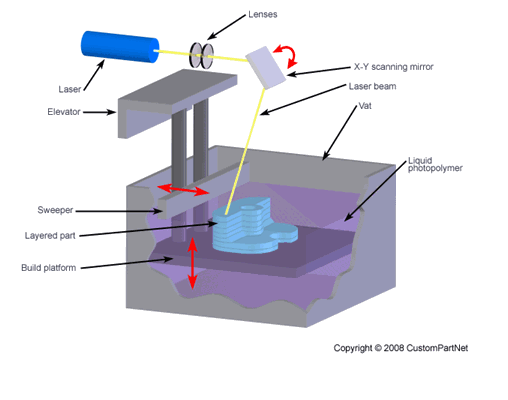
\includegraphics[scale=0.5]{build/Stereolithography.png}
\end{figure}


\subsection{Powder Bed Fusion}
Selective laser sintering (SLS) was one of the first additive manufacturing techniques, developed in the mid-1980s by Dr. Carl Deckard and Dr. Joe Beaman at the University of Texas at Austin. Their method has since been changed to work with a larger range of materials. This include plastics, metals, glass and other composite material powder. Today this is called Powder Bed Fusion. \\

Power bed fusion is the most common additive manufacturing technology for industrial applications. It starts by using a atomizer. Atomisation is the process of transforming a solid solution form into fine particles in a surrounding gas.  The end result is a powder which than can be used for 3D printing. \\

Industrial power bed fusion systems use a single or multiple high-power carbon dioxide lasers. Powder is dispersed in a thin layer on top of a platform inside  the build chamber.
The printer preheats the powder to a temperature just below the melting point. This makes it easier for the laser to raise the temperature of specific regions of the powder bed as it traces the model to solidify a part. This fuses the particles together mechanically to create one solid part.\\

It is most used in very specialized facilities and has very specific requirements to work properly though it is superior in its strength and for creating very large objects.  \\


\begin{figure}[hbtp]
\caption{Powder Bed Fusion}
\centering
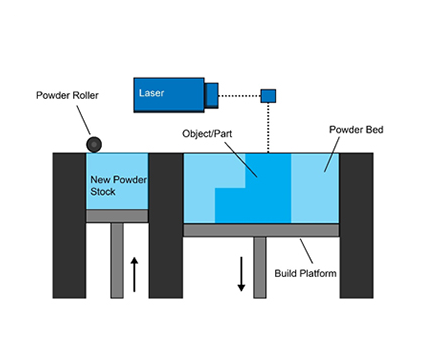
\includegraphics[scale=0.75]{PBF.png}
\end{figure}



\newpage


\subsection{Auger Design}

A auger design is based on the principles of the Archimedes screw. It is a machine  used for transferring water from a low-lying body of water into irrigation ditches. Water is pumped by turning a screw-shaped surface inside a pipe.  This technology has been around since Egyptian times, when it was used to remove water from the Nile river.\\

 An auger design uses a screw (auger) to move material down a cylinder. The rotation of the screw creates a shearing force on the material which drives it down the threads of the screw. A example of a 3d print auger design is shown below.\\
 
 \begin{figure}[hbtp]
 \caption{Auger}
 \centering
 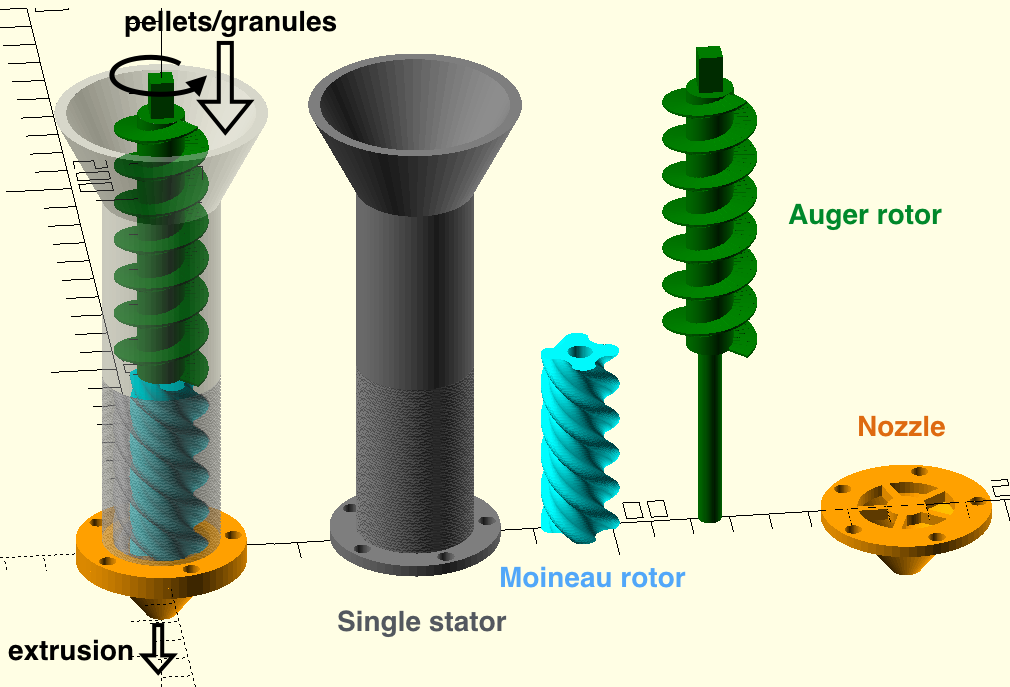
\includegraphics[scale=0.25]{auger.png}
 \end{figure}
 

 
  \subparagraph{Types of screw}
 There are many variations in the design of the screw which are fundamental in moving the fluid through. The primary differences consist of the number of intermeshing screws involved, the pitch of the screws, and the general direction of fluid flow. A single screw pump contains a single screw that rotates within a closed tube. The individual screw pushes a set volume of fluid forwards with every rotating. Two screws or more can benefit a precise flow rate but  come at the expense of high cost and additional maintenance. 
\\
 \begin{figure}[hbtp]
 \caption{Screw design}
 \centering
 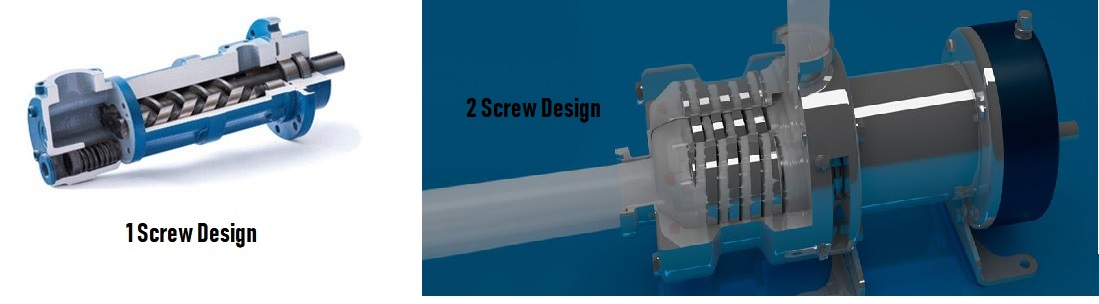
\includegraphics[scale=0.5]{screwCombine.png}
 \end{figure}
 





\newpage
 
 
\subsection{Auger Design + Fluid Pump Extruder}

 The  characteristics  of a fluid  pump  is  that by  adjusting  the  motor speed  you can control  the flow rate. It works by having a closed tube with at the end a cover which creates a airtight seal. This cover is connected to the motor which pushes it down through the tube.\\
 
  As the material is pushed down it comes in contact with the screw, which turns for a set length of time or rotates at a specified speed.  The screw is causing the material to move down the threads. As the material reaches the end of the nozzle the pressure  increases. This is due to the fact that the  flow  encounters resistance due to the restriction in area at the nozzle.\\
  
Any area restriction such as at the output of the auger creates backflow. The amount of backflow is proportional to the pressure drop from the nozzle to the extruder. As long as the the pressure inside the system is stable, the flow out of the needle is equal to the rotorspeed flow minus the backflow.   \\

With this design it is very import to control the pressure inside the system. 

\begin{itemize}
	\item Low Air pressure
	\begin{itemize}
		\item screw will cavitate
		\item create missed dots
		\item inconsistent 3D objects
	\end{itemize}
\end{itemize}

 \begin{itemize}
	\item High Air pressure
	\begin{itemize}
		\item Material will be forced through
		\item drool(excess of fluid)
		\item inconsistent 3D objects
	\end{itemize}
\end{itemize}

\begin{figure}[hbtp]
\caption{Auger \& Extruder}
\centering
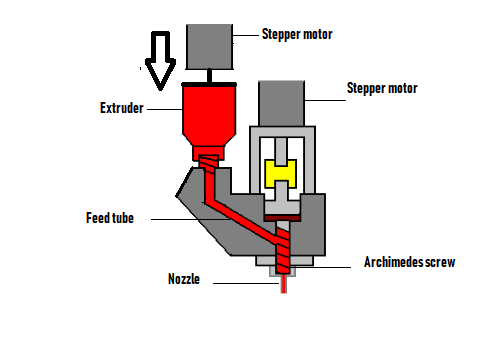
\includegraphics[scale=1]{augerAndExtruder.png}
\end{figure}


 \newpage
 \section{Motors}
	In this part of preliminary research we will look at the different kind of motors available. Every printer needs motors for the x \& y \& z  axis, futhermore the 3D printhead/extruder needs depending on the type also 1 or more motors. \\
	
	\subsection{Brush motor}
 		The DC brush motor is one of the simplest motors in use today. You can find these motors just about anywhere. They are in household appliances, toys, and automobiles. Being simple to construct and control, these motors are the go-to solution for professionals and hobbyists.\\
 		
 		If energy flows the windings are energized, they attract to the magnets located around the motor. This rotates the motor until the brushes make contact with a new set of  contacts. This new contact energizes a new set of windings and starts the process again.
 		
\begin{itemize}		
\item Pros
\begin{itemize}
		\item Simple to control
		\item Excellent torque at low RPM
		\item Inexpensive and mass produced
		\item Simple to control
	\end{itemize}		
\end{itemize}	


 
\begin{itemize}		
\item Cons
\begin{itemize}
		\item Brushes can wear out over time
		\item Brush arcing can generate electromagnetic noise
		\item  Usually limited in speed due to brush heating
	
	\end{itemize}		
\end{itemize}		

\begin{figure}[hbtp]
\caption{Brush motor }
\centering
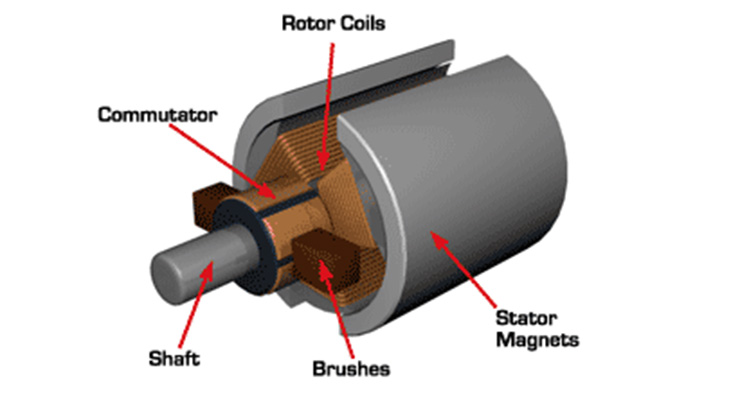
\includegraphics[scale=1]{build/brushMotor.png}
\end{figure} 		

\newpage

	\subsection{Brushless motor}
Brushless motors have begun to dominate the hobby markets between aircraft and ground vehicles. Controlling these motors was until a few years difficult due to the fact that controllers were buggy and expensive. Nowadays micro controllers are cheaper and powerful enough to handle the task. Without brushes to fail, these motors deliver more power and can do so more silently.\\

The mechanics of a brushless motor are simple. The only moving part is the the rotor, which contains the magnets. Where things become complicated is orchestrating the sequence of energizing windings. The polarity of each winding is controlled by the direction of current flow. 

\begin{itemize}		
\item Pros
\begin{itemize}
		\item Reliable
		\item High speed
		\item Efficient
		\item Mass produced and easy to find
	\end{itemize}		
\end{itemize}	 
 	
 				
\begin{itemize}		
\item Cons
\begin{itemize}
		\item Difficult to control without specialized controller
		\item Requires low starting loads
		\item Typically require specialized gearboxes in drive applications
	
	\end{itemize}		
\end{itemize}	

\begin{figure}[hbtp]
\caption{Brushless motor}
\centering
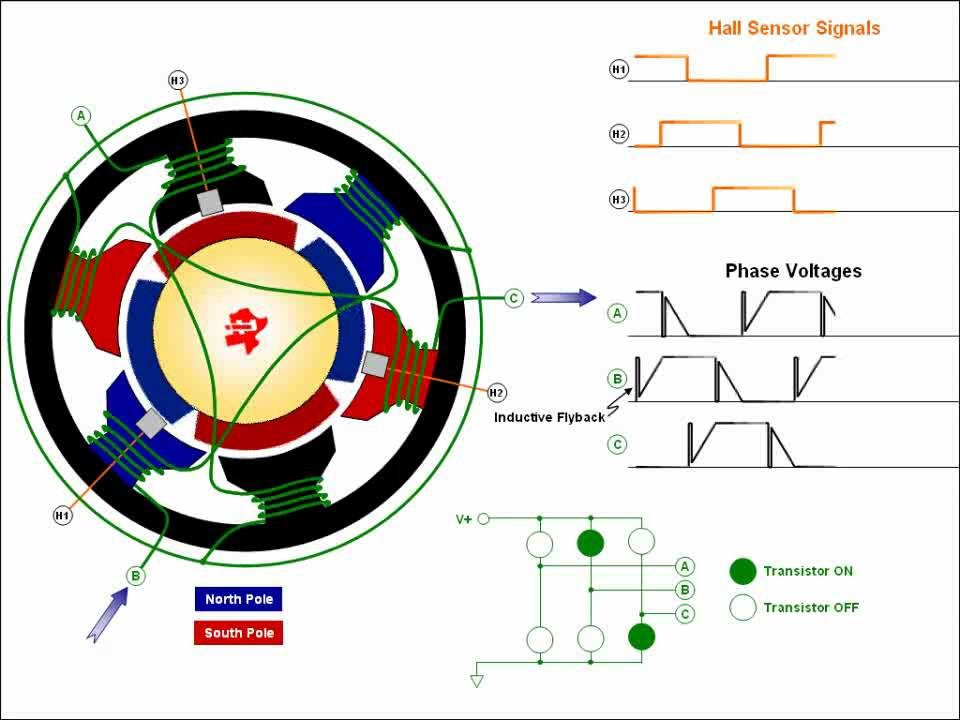
\includegraphics[scale=0.35]{build/brushless.png}
\end{figure}



\newpage


	\subsection{Stepper motor}
Stepper motors are  motors for position control. They can be found in desktop printers, plotters, CNC milling machines  and anything else requiring precise position control. Steppers are a special segment of brushless motors. They are purposely built for high-holding torque. This high-holding torque gives the user the ability to incrementally "step" to the next position. \\

Stepper motors behave exactly the same as a brushless motor, only the step size is much smaller. The only moving part is  the rotor, which contains the magnets. As with brushless motors the complicated aspect is orchestrating the sequence of the windings. 

\begin{itemize}		
\item Pros
\begin{itemize}
		\item Excellent position accuracy
		\item   High holding torque
		\item  High reliability
		\item   Most steppers come in standard sizes
	\end{itemize}		
\end{itemize}	 
 	
 				
\begin{itemize}		
\item Cons
\begin{itemize}
		\item Small step distance limits top speed
		\item    It's possible to "skip" steps with high loads
		\item    Draws maximum current constantly
	
	\end{itemize}		
\end{itemize}	
\begin{figure}[hbtp]
\caption{Steppermotor}
\centering
\includegraphics[scale=0.15]{build/Steppermotor.png}
\end{figure}

\newpage
\subsection{Linear motors }


A linear motor is often described as a rotary motor, just cut up and rolled out. Linear motors use magnetic levitation to move an object. This way it is not slowed down by friction and can actually achieve more precise control than mechanical options.\\

In a traditional electric motor, the rotor spins inside the stator. In a linear motor the stator is unwrapped and laid out flat and the "rotor" moves past it in a straight line. Linear motors have a number of advantages over ordinary motors. There are no moving parts to go wrong. As the platform rides above the track on a cushion of air, there is no loss of energy to friction or vibration. The same technique drives the Maglev trains.  

\begin{itemize}		
\item Pros
\begin{itemize}
		\item  Reliable
		\item  High speed
		\item  Efficient
		\item  No rotary to linear conversion required
	\end{itemize}		
\end{itemize}	 
 	
\begin{itemize}		
\item Cons
\begin{itemize}
		\item    Expensive
		\item    Require custom controllers
		\item    Purpose built for each system
	
	\end{itemize}		
\end{itemize}	
\begin{figure}[hbtp]
\caption{Linear motor}
\centering
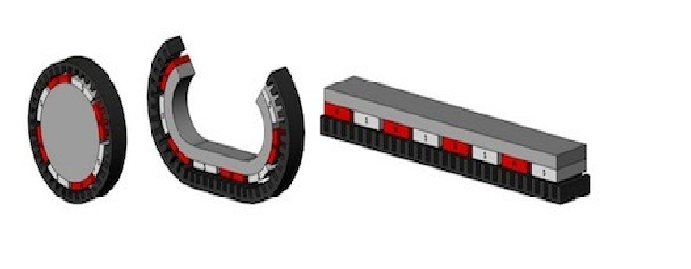
\includegraphics[scale=0.5]{build/linearMotor.png}
\end{figure}

\newpage
 
 
\section{Morphological Chart}
 	
 	\begin{center}
Table 1. Morphological chart
\end{center}
 \begin{center}
 \begin{tabular}{|| c || c | c | c | c ||}
 
 \hline\hline
    \textit{Sub Functions} & \textit{Solutions} & \textit{Solutions}  & \textit{Solutions} & \textit{Solutions}   \\ [1.5ex]  
  \hline\hline
   
   \textit{3D head Type} & Stereolithography & Power Bed Fusion &  Auger + Extruder &  Hotend    \\
   \hline
    \textit{Motor} & Brush motor & Stepper motor & Linear motor & Brushless motor   \\
   \hline

 	\textit{Screw type} & 1 Screw &  2 screw & x & x  \\
   \hline   
   	\textit{3D printhead material}   & ABS/PLA & Metal casting & Aluminum & Wood     \\
   	\hline
   	\textit{Nozzle size}  & 0.6  & 0.8 &  1.2  & 1.5   \\
   	\hline 
   	\textit{Controller}  & Mega + RAMPS & Smoothieboard & Azteeg X5 GT  & RADDS   \\
   	\hline\hline 
   
   
 \end{tabular}
\end{center}  

\section{Are there already existing (partial) solutions to this problem? }
For the Playaprinter the  objectives are to create a massive 3D printer that can print with natural resources. The choice for this project is based on clay or other materials with a similar liquid properties. It needs to be fabricated with normal purchasable parts without resorting to expensive solutions. Furthermore it needs to print large 3D objects with a high level of detail.  \\

 Currently the are no (affordable) clay printer purchasable. The are a few clay nozzle sets and extruders but for a very steep price and with questionable performance. The also come bundled with closed software and are meant for small printing. \\ 
 
 So it will be required to make a custom solution that satisfies the needs for this project. This will include the 3D print head which receives the clay and hold the auger and motor. The nozzle will be attach to the bottom of the 3D head which will feed the clay. \\
 
 
 With regards to the other parts:
 
 	\begin{itemize}
 		\item Nozzle size
 		\item Controller
	\end{itemize} 	 
 
In these categories the are several parts available to purchase. It will be a combination of desk research and field research to determine the best combination of components. After this process the need to be combined through soldering and creating code for all the individual component necessary.
 \newpage
 
 
\section{Conclusion }

Playaprinter needs to be a printer that is able to print material over a large x \& y \& z axis, with a 3D head + nozzle that is capable to print clay with a high level of detail. \\

 The playaprinter will need a auger + extruder design to function correctly. This is because of the sheer pressure required to push the clay through.\\
 
  The extruder can push the clay in which the extruder is essential. In combination with a auger design it should be possible to print clay. The combination of a auger and extruder should ensure a system in which a double system of delivery  works together. The auger creates a high pressure zone in which the clay is pressed through the nozzle whilst the extruder controls the overall system pressure. \\

 With the combination of a auger and a extruder the accuracy of the 3D print should increase. It can solve outflow problems due to the fact that pressure inside is controlled and should result in a smooth and accurate 3D printed object. \\
 
It will require creating several custom 3D printed objects to craft all the necessary parts.   Also needed is a workshop to create and lay out all the parts.\\

 Beside the fact that a 3D printer is needed for the project, a laser cutter is very useful for easy and fast prototyping. The material for the frame while be aluminum. The is because of the lightweight and sturdy properties. \\
 
 The frame that will support the 3D head also needs to be created. It needs to be flexible in design so that in the future it can be easily replaced or swap with a more traditional hotend or other designs. Futhermore it needs to able to withstand all the stresses and weight from the clay extruder.\\
 
 Lastly the motors that will be used are steppermotors. The reason for this is that we need a high level of accuracy. One of the most important aspect will be to generate enough torque. A normal steppermotor can't deliver enough torque to push clay through. A additional gearbox or gear conversion is needed to maintain the best combination of torque and speed. 

 	\begin{center}
Table 2. Morphological chart with part selection
\end{center}
 \begin{center}
 \begin{tabular}{|| c || c | c | c | c ||}
 
 \hline\hline
    \textit{Sub Functions} & \textit{Solutions} & \textit{Solutions}  & \textit{Solutions} & \textit{Solutions}   \\ [1.5ex]  
  \hline\hline
   
   \textit{3D head Type} & Stereolithography & Power Bed Fusion & \textcolor{green}{ Auger + Extruder} &  Hotend    \\
   \hline
    \textit{Motor} & Brush motor & \textcolor{green}{Stepper motor} & Linear motor & Brushless motor   \\
   \hline

 	\textit{Screw type} & \textcolor{green}{1 Screw} &  2 screw & x & x  \\
   \hline   
   	\textit{3D printhead material}   & \textcolor{green}{ ABS/PLA }& Metal casting & Aluminum & Wood     \\
   	\hline
   	\textit{Nozzle size}  & 0.6  & 0.8 & \textcolor{green}{ 1.2}  &\textcolor{green}{ 1.5 }  \\
   	\hline 
   	\textit{Controller}  & \textcolor{green}{ Mega + RAMPS } & Smoothieboard & Azteeg X5 GT  & RADDS   \\
   	\hline\hline 
   
   
 \end{tabular}
\end{center}  

\newpage

\section{Bills of Materials}

These items are necessary to create the 3D head and create a 3D design that works with clay  extruder.  

\begin{itemize}
	\item 3D Printhead
	\begin{itemize}
		\item Printed 3D Head(needs to be printed)
		\item Printed Base (needs to be printed)
		\item Nema 17 stepper motor 
		\item Stepper driver A4988
		\item Mega 2560 + RAMPS 1.4
		\item 1/2" Flat faucet washer
		\item 3/8" x 3/8" push fit male adapter
		\item Aluminum coupler 5mm
		\item Deck Screw	
		\item Cake decorating tips (nozzle)
		\item Acces to wood/metal for creating frames and support structures. 
	\end{itemize}
	\item Extruder
	\begin{itemize}
		\item 3D parts (needs to be printed)
		\item Nema 23 stepper motor 
		\item Stepper driver A4988
		\item Nema 23 gearbox: either 20:1 or 30:1
		\item Leadscrew
		\item Acces to wood/metal for creating frames and support structures. 		
	\end{itemize}	
\end{itemize}

	
	
\newpage
    
   
\section{Sources}
	

		University of Notre Dame.(2013). Initial Extruder Design. Accessed at 25 February 2019, from \\
	https://sites.nd.edu/3dp/2013/08/12/initial-extruder-design/\\
	
		The Italian Associationof Chemical Engineering.(2017). Design of 3D Metal FDM Printing Nozzle 	Based on Melt Forming. Accessed at 25 2019, from \\ 
	https://www.aidic.it/cet/17/59/013.pdf/ \\
	
		www.manufactur3dmag.com.(2018). 7 Methods of Manufacturing Metal 3D Printing Powder. Accessed at 25 			February 2019, from \\
	https://manufactur3dmag.com/7-methods-manufacturing-metal-3d-printing-powder/\\
		
	www.engineersedge.com (2018). Screw Type Positive Displacement Pump . Accessed at 25 February 2019, from \\
	http://beta.briefideas.org/ideas/ae254dc0e368a1b2b87b4047109f9b59\\
	
	Colfax Fluid HandlingWhite Paper.(2011). What’s a screw pump? Understanding the unique characteristics and operating principles of 1, 2 and 3 screw pumps. Accessed at  25 February 2019, from \\
	http://empoweringpumps.com/wp-content/uploads/sites/3/2013/05/What-is-a-screw-pump.pdf\\
	
	www.engineersedge.com (2018). Screw Type Positive Displacement Pump . Accessed at 25 February 2019, from \\
	http://beta.briefideas.org/ideas/ae254dc0e368a1b2b87b4047109f9b59\\
	
		Ali Morris, Dezeen.com .(2018). Dutch designers convert algae into bioplastic for 3D printing. Accessed at 25 February 2019, from \\
	https://www.dezeen.com/2017/12/04/dutch-designers-eric-klarenbeek-maartje-dros-convert-algae-biopolymer-3d-printing-good-design-bad-world/	\\
	
		www.3ders.org.(2013). 3D printed 'Mycelium Chair' made from water, straw and fungus. Accessed at 25 February 2019, from \\
	https://www.3ders.org/articles/20131021-3d-printed-mycelium-chair-made-from-water-straw-and-fungus.html\\
	
		3D Printlife.(2018). ALGA™ Algae Based PLA. Accessed at 25 February 2019, from \\
	https://www.3dprintlife.com/http/www3dprintlifecom/filaments/alga\\
	
	Wageningen University \& Research.(2016). MACROFUELS: Macro-algae as a sustainable source for biofuels. Accessed at 25 February 2019, from \\
	https://www.wur.nl/nl/project/MACROFUELS-Macro-algae-as-a-sustainable-source-for-biofuels.html\\
	
	Menno\-Jan\_Rietema\, University of Twente.(2015). Design of a prototype machine for 3D printing with continous fibre. Accessed at 25 February 2019, from \\
	https://essay.utwente.nl/71622/1/Thesis\_Menno\-Jan\_Rietema.pdf\\
	
	Tom Landerhaus.(2018). Bricoleur Clay Extruder, Open Source. Accessed at 25 February 2019, from \\
	https://www.thingiverse.com/thing:1413969\\
	
		Bryan Cera.(2018). Bricoleur Clay Extruder. Accessed at 25 February 2019, from \\ 
	https://www.thingiverse.com/thing:1413969\\
	
\newpage	
	 	Wikipedia(2018). Clay. Accessed at 25 February 2019, from \\ 
	https://en.wikipedia.org/wiki/Clay\\
	
	 	Formlabs.com. (2018). FDM vs SLA vs SLS . Accessed at 25 February 2019, from \\ 
     https://formlabs.com/blog/fdm-vs-sla-vs-sls-how-to-choose-the-right-3d-printing-technology/\\
	
		Formlabs.com.(2018). Ultimate guide tot stereolithography . Accessed at 25 February 2019, from \\ 
	https://formlabs.com/blog/ultimate-guide-to-stereolithography-sla-3d-printing/\\
	
		Wikipedia.(2018). Photopolymer. Accessed at 25 February 2019, from \\ 
	https://en.wikipedia.org/wiki/Photopolymer\\
	
		Loughborough University.(2018). Powder Bed Fusion . Accessed at 25 February 2019, from \\ 
	https://www.lboro.ac.uk/research/amrg/about/the7categoriesofadditivemanufacturing/powderbedfusion/\\

	
	    M. Entezarian F. Allaire P. TsantrizosR. A.L.DrewBryan.(1996). Plasma atomization: A new process for the production of fine, spherical powders. Accessed at 25 February 2019, from \\ 
	https://link.springer.com/article/10.1007/BF03222969\\
	
		Motioncontroltips.com (2017).  How can brush wear in DC motors be minimized?. Accessed at 25 February 2019, from \\ 
	https://www.motioncontroltips.com/faq-how-can-brush-wear-in-dc-motors-be-minimized/\\
	
	
		Motioncontroltips.com (2017).  linear motor how it works. Accessed at 25 February 2019, from \\ 	
	https://www.motioncontrol.com/products/linear-motor-how-it-works/\\
	
	www.applied-motion.com (2018). What do nema suzes meen. Accessed at 25 February 2019, from \\ 
     https://www.applied-motion.com/news/2015/10/what-do-nema-sizes-mean\\
	
	www.applied-motion.com (2018). Gear stacks. Accessed at 25 February 2019, from \\ 
	https://www.applied-motion.com/news/2015/10/stacks-stacks
	
	
\end{document}



 

